%%%%%%%%%%%%%%%%%%%%%%%%%%%%%%%%%%%%%%%%%%%%%%%%%%%%%%%%%%%%%%%%%%%%%%%%%%%%%%%%%%%%%%%%%%%%%%%%%%%%%%%%%%%%%%%%%%%%%%%%%%%%%%%%%%%%%%%%%%%%%%%%%%%%%%%%%%%%%%%%%%%
% Written By Michael Brodskiy
% Class: Cornerstone Engineering 1 & 2 (GE1501 & GE1502)
% Professor: B. O'Connell
%%%%%%%%%%%%%%%%%%%%%%%%%%%%%%%%%%%%%%%%%%%%%%%%%%%%%%%%%%%%%%%%%%%%%%%%%%%%%%%%%%%%%%%%%%%%%%%%%%%%%%%%%%%%%%%%%%%%%%%%%%%%%%%%%%%%%%%%%%%%%%%%%%%%%%%%%%%%%%%%%%%

\include{Includes.tex}

\title{Algorithmic Thinking and Representations Homework}
\date{\today}
\author{Michael Brodskiy\\ \small Professor: B. O'Connell}

\begin{document}

\maketitle

\listoffigures

\begin{enumerate}

    \newpage

  \item Marble Flowchart:

    \begin{figure}[H]
      \centering \tikzset{every picture/.style={line width=0.75pt}} %set default line width to 0.75pt        

\begin{tikzpicture}[x=0.75pt,y=0.75pt,yscale=-1,xscale=1]
%uncomment if require: \path (0,812); %set diagram left start at 0, and has height of 812

%Shape: Ellipse [id:dp7078776640454232] 
\draw   (270,32) .. controls (270,18.75) and (293.28,8) .. (322,8) .. controls (350.72,8) and (374,18.75) .. (374,32) .. controls (374,45.25) and (350.72,56) .. (322,56) .. controls (293.28,56) and (270,45.25) .. (270,32) -- cycle ;
%Shape: Boxed Line [id:dp972704207942342] 
\draw    (322,56) -- (322,133) ;
\draw [shift={(322,135)}, rotate = 270] [color={rgb, 255:red, 0; green, 0; blue, 0 }  ][line width=0.75]    (10.93,-3.29) .. controls (6.95,-1.4) and (3.31,-0.3) .. (0,0) .. controls (3.31,0.3) and (6.95,1.4) .. (10.93,3.29)   ;
%Flowchart: Process [id:dp12474322255758397] 
\draw   (252,134) -- (393,134) -- (393,204) -- (252,204) -- cycle ;
%Shape: Boxed Line [id:dp03382264465030782] 
\draw    (8,242) -- (319.71,237.03) ;
\draw [shift={(321.71,237)}, rotate = 179.09] [color={rgb, 255:red, 0; green, 0; blue, 0 }  ][line width=0.75]    (10.93,-3.29) .. controls (6.95,-1.4) and (3.31,-0.3) .. (0,0) .. controls (3.31,0.3) and (6.95,1.4) .. (10.93,3.29)   ;
%Shape: Boxed Line [id:dp28644614408481495] 
\draw    (323,203) -- (323,280) ;
\draw [shift={(323,282)}, rotate = 270] [color={rgb, 255:red, 0; green, 0; blue, 0 }  ][line width=0.75]    (10.93,-3.29) .. controls (6.95,-1.4) and (3.31,-0.3) .. (0,0) .. controls (3.31,0.3) and (6.95,1.4) .. (10.93,3.29)   ;
%Flowchart: Process [id:dp9898963336751274] 
\draw   (252,282) -- (393,282) -- (393,352) -- (252,352) -- cycle ;
%Flowchart: Decision [id:dp6216008434832396] 
\draw   (322,432) -- (391,474) -- (322,516) -- (253,474) -- cycle ;
%Shape: Boxed Line [id:dp7931040026577363] 
\draw    (322,353) -- (322,430) ;
\draw [shift={(322,432)}, rotate = 270] [color={rgb, 255:red, 0; green, 0; blue, 0 }  ][line width=0.75]    (10.93,-3.29) .. controls (6.95,-1.4) and (3.31,-0.3) .. (0,0) .. controls (3.31,0.3) and (6.95,1.4) .. (10.93,3.29)   ;
%Shape: Boxed Line [id:dp6715019356060254] 
\draw    (253,474) -- (176,474) ;
\draw [shift={(174,474)}, rotate = 360] [color={rgb, 255:red, 0; green, 0; blue, 0 }  ][line width=0.75]    (10.93,-3.29) .. controls (6.95,-1.4) and (3.31,-0.3) .. (0,0) .. controls (3.31,0.3) and (6.95,1.4) .. (10.93,3.29)   ;
%Shape: Boxed Line [id:dp45065332069120023] 
\draw    (391,474) -- (468,474) ;
\draw [shift={(470,474)}, rotate = 180] [color={rgb, 255:red, 0; green, 0; blue, 0 }  ][line width=0.75]    (10.93,-3.29) .. controls (6.95,-1.4) and (3.31,-0.3) .. (0,0) .. controls (3.31,0.3) and (6.95,1.4) .. (10.93,3.29)   ;
%Flowchart: Process [id:dp8374841194029297] 
\draw   (469,439) -- (610,439) -- (610,509) -- (469,509) -- cycle ;
%Flowchart: Process [id:dp16793270470552768] 
\draw   (33,439) -- (174,439) -- (174,509) -- (33,509) -- cycle ;
%Flowchart: Decision [id:dp8898317341435751] 
\draw   (325,628) -- (394,670) -- (325,712) -- (256,670) -- cycle ;
%Straight Lines [id:da18982359592399445] 
\draw    (540,510) -- (354.62,643.83) ;
\draw [shift={(353,645)}, rotate = 324.17] [color={rgb, 255:red, 0; green, 0; blue, 0 }  ][line width=0.75]    (10.93,-3.29) .. controls (6.95,-1.4) and (3.31,-0.3) .. (0,0) .. controls (3.31,0.3) and (6.95,1.4) .. (10.93,3.29)   ;
%Shape: Boxed Line [id:dp7328385757826796] 
\draw    (107,508) -- (291.39,644.81) ;
\draw [shift={(293,646)}, rotate = 216.57] [color={rgb, 255:red, 0; green, 0; blue, 0 }  ][line width=0.75]    (10.93,-3.29) .. controls (6.95,-1.4) and (3.31,-0.3) .. (0,0) .. controls (3.31,0.3) and (6.95,1.4) .. (10.93,3.29)   ;
%Shape: Boxed Line [id:dp04108068314750124] 
\draw    (394,670) -- (471,670) ;
\draw [shift={(473,670)}, rotate = 180] [color={rgb, 255:red, 0; green, 0; blue, 0 }  ][line width=0.75]    (10.93,-3.29) .. controls (6.95,-1.4) and (3.31,-0.3) .. (0,0) .. controls (3.31,0.3) and (6.95,1.4) .. (10.93,3.29)   ;
%Shape: Boxed Line [id:dp2583793005729782] 
\draw    (256,670) -- (9,671) ;
%Shape: Boxed Line [id:dp07004372573074047] 
\draw    (8,242) -- (9,671) ;
%Flowchart: Terminator [id:dp5241120411854552] 
\draw   (495.08,642) -- (588.92,642) .. controls (601.11,642) and (611,654.54) .. (611,670) .. controls (611,685.46) and (601.11,698) .. (588.92,698) -- (495.08,698) .. controls (482.89,698) and (473,685.46) .. (473,670) .. controls (473,654.54) and (482.89,642) .. (495.08,642) -- cycle ;

% Text Node
\draw (322,32) node   [align=left] {Draw Marble};
% Text Node
\draw (322.5,169) node   [align=left] {Set aside as largest};
% Text Node
\draw (322.5,317) node   [align=left] {Draw new marble};
% Text Node
\draw (280,455) node [anchor=north west][inner sep=0.75pt]   [align=left] {Larger than\\ old marble?};
% Text Node
\draw (206,462.5) node [anchor=west] [inner sep=0.75pt]   [align=left] {yes};
% Text Node
\draw (418,456) node [anchor=north west][inner sep=0.75pt]   [align=left] {no};
% Text Node
\draw (539.5,474) node   [align=left] {Discard new marble};
% Text Node
\draw (103.5,474) node   [align=left] {Discard old marble\\Set aside new one};
% Text Node
\draw (328.93,674) node   [align=left] {\begin{minipage}[lt]{67.9pt}\setlength\topsep{0pt}
\begin{center}
More marbles \\in bag?
\end{center}

\end{minipage}};
% Text Node
\draw (115,658.5) node [anchor=west] [inner sep=0.75pt]   [align=left] {yes};
% Text Node
\draw (421,652) node [anchor=north west][inner sep=0.75pt]   [align=left] {no};
% Text Node
\draw (542,670) node   [align=left] {Largest marble\\is set aside};


\end{tikzpicture}

      \caption{Flowchart for Drawing the Largest Marble}
      \label{fig:1}
    \end{figure}

    \newpage

  \item Rock Paper Scissors Pseudocode:

    \begin{algorithm}
      \caption{Rock, Paper, Scissors}\label{RPS}
      \begin{algorithmic}[1]
        \Procedure{Rock Paper Scissors}{}
        \State Players (P1 \& P2) Throw Hands;
        \If {P1 has rock}
            \If {P2 has scissors} P1 wins; $\rightarrow$ Game ends;
            \ElsIf {P2 has paper} P2 wins; $\rightarrow$ Game ends;
            \Else { Tie; $\rightarrow$ Play again;}
        \EndIf
        \ElsIf {P1 has scissors}
            \If {P2 has paper} P1 Wins; $\rightarrow$ Game ends;
            \ElsIf {P2 has rock} P2 Wins; $\rightarrow$ Game ends;
            \Else { Tie; $\rightarrow$ Play again;}
        \EndIf
        \Else
            \If {P2 has rock} P1 Wins; $\rightarrow$ Game ends;
            \ElsIf{P2 has scissors} P2 Wins; $\rightarrow$ Game ends;
            \Else { Tie; $\rightarrow$ Play again;}
        \EndProcedure
      \end{algorithmic}
    \end{algorithm}

    \newpage

  \item Blackjack Dealer Flowchart for $n$ players:

    \begin{figure}[H]
      \centering \tikzset{every picture/.style={line width=0.75pt}} %set default line width to 0.75pt        

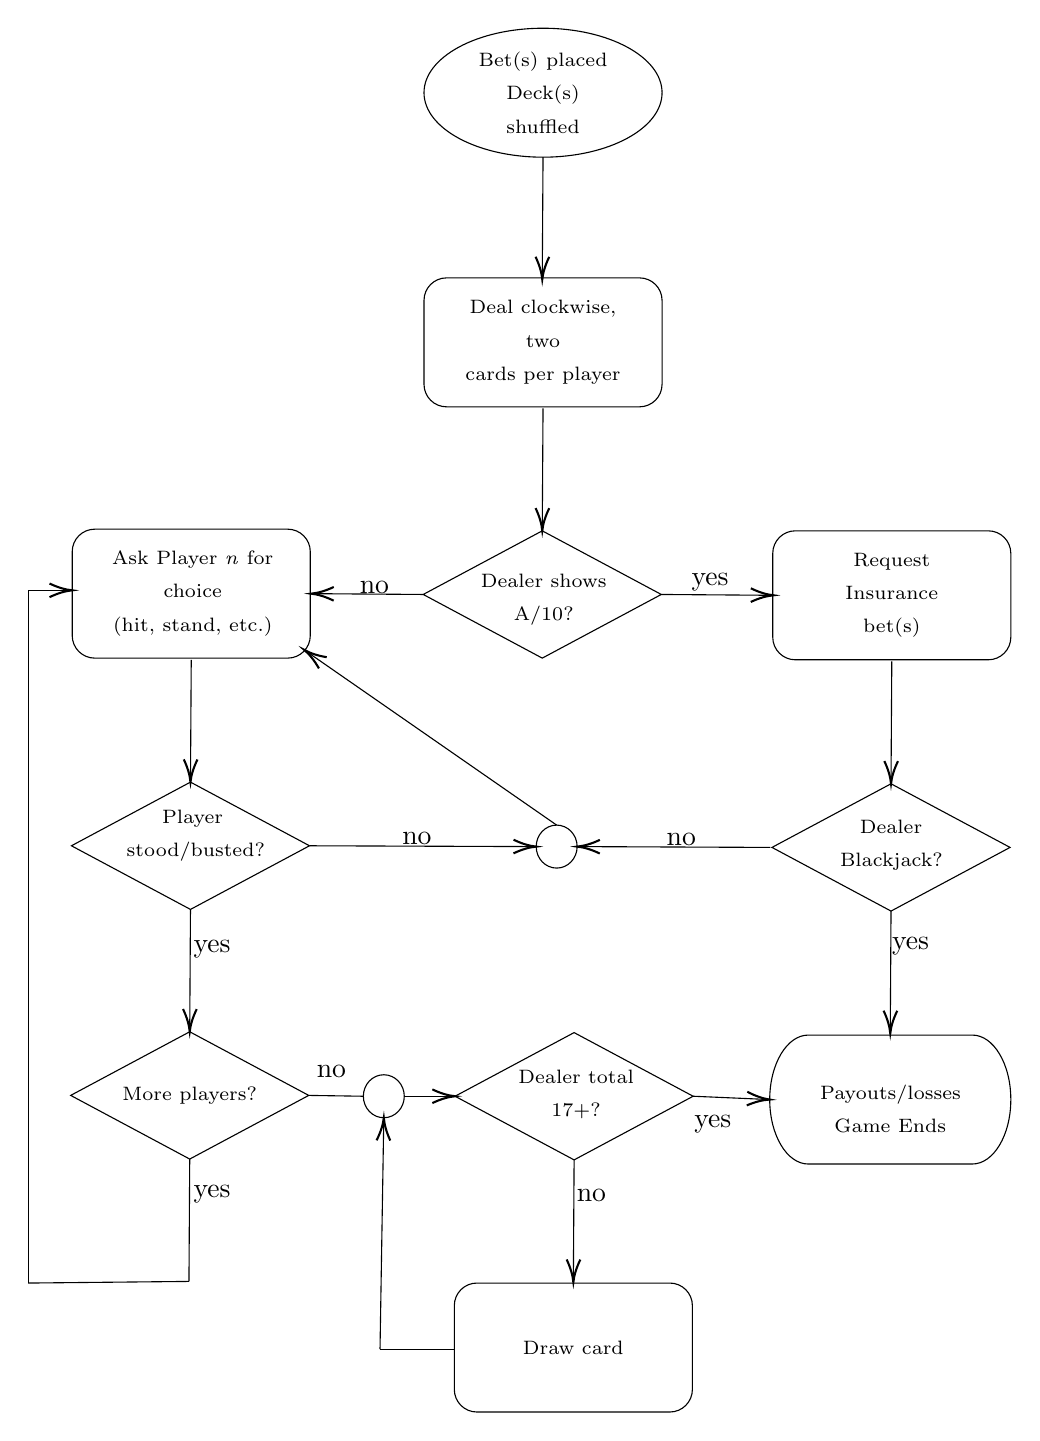
\begin{tikzpicture}[x=0.75pt,y=0.75pt,yscale=-1,xscale=1]
%uncomment if require: \path (0,879); %set diagram left start at 0, and has height of 879

%Shape: Ellipse [id:dp29724360855055476] 
\draw   (283.68,38.06) .. controls (283.68,20.91) and (309.35,7) .. (341.03,7) .. controls (372.7,7) and (398.38,20.91) .. (398.38,38.06) .. controls (398.38,55.22) and (372.7,69.13) .. (341.03,69.13) .. controls (309.35,69.13) and (283.68,55.22) .. (283.68,38.06) -- cycle ;
%Shape: Boxed Line [id:dp10915548988637624] 
\draw    (341.03,69.13) -- (340.67,126.07) ;
\draw [shift={(340.66,128.07)}, rotate = 270.36] [color={rgb, 255:red, 0; green, 0; blue, 0 }  ][line width=0.75]    (10.93,-3.29) .. controls (6.95,-1.4) and (3.31,-0.3) .. (0,0) .. controls (3.31,0.3) and (6.95,1.4) .. (10.93,3.29)   ;
%Flowchart: Alternative Process [id:dp4643848333429237] 
\draw   (283.68,138.15) .. controls (283.68,132.14) and (288.55,127.28) .. (294.55,127.28) -- (387.5,127.28) .. controls (393.51,127.28) and (398.38,132.14) .. (398.38,138.15) -- (398.38,178.53) .. controls (398.38,184.54) and (393.51,189.41) .. (387.5,189.41) -- (294.55,189.41) .. controls (288.55,189.41) and (283.68,184.54) .. (283.68,178.53) -- cycle ;
%Flowchart: Decision [id:dp7527013815159744] 
\draw   (340.66,249.15) -- (398.01,279.81) -- (340.66,310.48) -- (283.31,279.81) -- cycle ;
%Shape: Boxed Line [id:dp9804992059437565] 
\draw    (341.03,190.2) -- (340.67,247.15) ;
\draw [shift={(340.66,249.15)}, rotate = 270.36] [color={rgb, 255:red, 0; green, 0; blue, 0 }  ][line width=0.75]    (10.93,-3.29) .. controls (6.95,-1.4) and (3.31,-0.3) .. (0,0) .. controls (3.31,0.3) and (6.95,1.4) .. (10.93,3.29)   ;
%Shape: Boxed Line [id:dp47497876735478184] 
\draw    (398.01,279.81) -- (450.07,280.2) ;
\draw [shift={(452.07,280.21)}, rotate = 180.42] [color={rgb, 255:red, 0; green, 0; blue, 0 }  ][line width=0.75]    (10.93,-3.29) .. controls (6.95,-1.4) and (3.31,-0.3) .. (0,0) .. controls (3.31,0.3) and (6.95,1.4) .. (10.93,3.29)   ;
%Shape: Boxed Line [id:dp3018054573423514] 
\draw    (283.31,279.81) -- (231.25,279.43) ;
\draw [shift={(229.25,279.42)}, rotate = 0.42] [color={rgb, 255:red, 0; green, 0; blue, 0 }  ][line width=0.75]    (10.93,-3.29) .. controls (6.95,-1.4) and (3.31,-0.3) .. (0,0) .. controls (3.31,0.3) and (6.95,1.4) .. (10.93,3.29)   ;
%Flowchart: Alternative Process [id:dp3713314658929583] 
\draw   (451.71,260.02) .. controls (451.71,254.02) and (456.58,249.15) .. (462.58,249.15) -- (555.53,249.15) .. controls (561.54,249.15) and (566.41,254.02) .. (566.41,260.02) -- (566.41,300.4) .. controls (566.41,306.41) and (561.54,311.28) .. (555.53,311.28) -- (462.58,311.28) .. controls (456.58,311.28) and (451.71,306.41) .. (451.71,300.4) -- cycle ;
%Shape: Boxed Line [id:dp5782580025276254] 
\draw    (509.06,312.07) -- (508.7,369.02) ;
\draw [shift={(508.69,371.02)}, rotate = 270.36] [color={rgb, 255:red, 0; green, 0; blue, 0 }  ][line width=0.75]    (10.93,-3.29) .. controls (6.95,-1.4) and (3.31,-0.3) .. (0,0) .. controls (3.31,0.3) and (6.95,1.4) .. (10.93,3.29)   ;
%Flowchart: Decision [id:dp11985708552247054] 
\draw   (508.69,371.02) -- (566.04,401.68) -- (508.69,432.35) -- (451.34,401.68) -- cycle ;
%Shape: Boxed Line [id:dp9914171110695695] 
\draw    (508.69,432.35) -- (508.34,489.29) ;
\draw [shift={(508.33,491.29)}, rotate = 270.36] [color={rgb, 255:red, 0; green, 0; blue, 0 }  ][line width=0.75]    (10.93,-3.29) .. controls (6.95,-1.4) and (3.31,-0.3) .. (0,0) .. controls (3.31,0.3) and (6.95,1.4) .. (10.93,3.29)   ;
%Flowchart: Terminator [id:dp899034840826713] 
\draw   (468.83,492.09) -- (547.82,492.09) .. controls (558.09,492.09) and (566.41,506) .. (566.41,523.16) .. controls (566.41,540.31) and (558.09,554.22) .. (547.82,554.22) -- (468.83,554.22) .. controls (458.57,554.22) and (450.25,540.31) .. (450.25,523.16) .. controls (450.25,506) and (458.57,492.09) .. (468.83,492.09) -- cycle ;
%Shape: Boxed Line [id:dp22015135714416068] 
\draw    (450.61,401.68) -- (359.46,401.29) ;
\draw [shift={(357.46,401.29)}, rotate = 0.24] [color={rgb, 255:red, 0; green, 0; blue, 0 }  ][line width=0.75]    (10.93,-3.29) .. controls (6.95,-1.4) and (3.31,-0.3) .. (0,0) .. controls (3.31,0.3) and (6.95,1.4) .. (10.93,3.29)   ;
%Flowchart: Decision [id:dp35829958706775633] 
\draw   (171.17,370.22) -- (228.52,400.89) -- (171.17,431.55) -- (113.82,400.89) -- cycle ;
%Shape: Boxed Line [id:dp7878781531347581] 
\draw    (171.54,311.28) -- (171.18,368.22) ;
\draw [shift={(171.17,370.22)}, rotate = 270.36] [color={rgb, 255:red, 0; green, 0; blue, 0 }  ][line width=0.75]    (10.93,-3.29) .. controls (6.95,-1.4) and (3.31,-0.3) .. (0,0) .. controls (3.31,0.3) and (6.95,1.4) .. (10.93,3.29)   ;
%Shape: Boxed Line [id:dp9454430491131107] 
\draw    (171.17,431.55) -- (170.82,488.5) ;
\draw [shift={(170.81,490.5)}, rotate = 270.36] [color={rgb, 255:red, 0; green, 0; blue, 0 }  ][line width=0.75]    (10.93,-3.29) .. controls (6.95,-1.4) and (3.31,-0.3) .. (0,0) .. controls (3.31,0.3) and (6.95,1.4) .. (10.93,3.29)   ;
%Shape: Boxed Line [id:dp9813437863594172] 
\draw    (228.52,400.89) -- (335.74,401.28) ;
\draw [shift={(337.74,401.29)}, rotate = 180.21] [color={rgb, 255:red, 0; green, 0; blue, 0 }  ][line width=0.75]    (10.93,-3.29) .. controls (6.95,-1.4) and (3.31,-0.3) .. (0,0) .. controls (3.31,0.3) and (6.95,1.4) .. (10.93,3.29)   ;
%Straight Lines [id:da9202532634393268] 
\draw    (347.6,390.93) -- (227.61,307.64) ;
\draw [shift={(225.96,306.5)}, rotate = 34.77] [color={rgb, 255:red, 0; green, 0; blue, 0 }  ][line width=0.75]    (10.93,-3.29) .. controls (6.95,-1.4) and (3.31,-0.3) .. (0,0) .. controls (3.31,0.3) and (6.95,1.4) .. (10.93,3.29)   ;
%Flowchart: Decision [id:dp9022248173242242] 
\draw   (170.81,490.5) -- (228.15,521.16) -- (170.81,551.83) -- (113.46,521.16) -- cycle ;
%Shape: Boxed Line [id:dp9687591434950271] 
\draw    (274.18,521.56) -- (296.65,521.56) ;
\draw [shift={(298.65,521.56)}, rotate = 180] [color={rgb, 255:red, 0; green, 0; blue, 0 }  ][line width=0.75]    (10.93,-3.29) .. controls (6.95,-1.4) and (3.31,-0.3) .. (0,0) .. controls (3.31,0.3) and (6.95,1.4) .. (10.93,3.29)   ;
%Shape: Boxed Line [id:dp7579040436342506] 
\draw    (170.81,551.83) -- (170.44,610.78) ;
%Shape: Boxed Line [id:dp906195448221869] 
\draw    (170.44,610.78) -- (93,611.57) ;
%Straight Lines [id:da4179608814144966] 
\draw    (93,277.82) -- (93,611.57) ;
%Straight Lines [id:da28040587832595176] 
\draw    (93,277.82) -- (112.19,277.82) ;
\draw [shift={(114.19,277.82)}, rotate = 180] [color={rgb, 255:red, 0; green, 0; blue, 0 }  ][line width=0.75]    (10.93,-3.29) .. controls (6.95,-1.4) and (3.31,-0.3) .. (0,0) .. controls (3.31,0.3) and (6.95,1.4) .. (10.93,3.29)   ;
%Flowchart: Alternative Process [id:dp9788290403613216] 
\draw   (114.19,259.22) .. controls (114.19,253.22) and (119.05,248.35) .. (125.06,248.35) -- (218.01,248.35) .. controls (224.02,248.35) and (228.89,253.22) .. (228.89,259.22) -- (228.89,299.61) .. controls (228.89,305.61) and (224.02,310.48) .. (218.01,310.48) -- (125.06,310.48) .. controls (119.05,310.48) and (114.19,305.61) .. (114.19,299.61) -- cycle ;
%Flowchart: Decision [id:dp2482767103787895] 
\draw   (356,490.9) -- (413.35,521.56) -- (356,552.23) -- (298.65,521.56) -- cycle ;
%Shape: Boxed Line [id:dp8073196300493868] 
\draw    (413.35,521.56) -- (448.25,523.07) ;
\draw [shift={(450.25,523.16)}, rotate = 182.47] [color={rgb, 255:red, 0; green, 0; blue, 0 }  ][line width=0.75]    (10.93,-3.29) .. controls (6.95,-1.4) and (3.31,-0.3) .. (0,0) .. controls (3.31,0.3) and (6.95,1.4) .. (10.93,3.29)   ;
%Flowchart: Connector [id:dp6155672319322512] 
\draw   (337.74,401.29) .. controls (337.74,395.57) and (342.16,390.93) .. (347.6,390.93) .. controls (353.05,390.93) and (357.46,395.57) .. (357.46,401.29) .. controls (357.46,407) and (353.05,411.64) .. (347.6,411.64) .. controls (342.16,411.64) and (337.74,407) .. (337.74,401.29) -- cycle ;
%Flowchart: Connector [id:dp1022044890813949] 
\draw   (254.46,521.56) .. controls (254.46,515.84) and (258.87,511.21) .. (264.32,511.21) .. controls (269.76,511.21) and (274.18,515.84) .. (274.18,521.56) .. controls (274.18,527.28) and (269.76,531.92) .. (264.32,531.92) .. controls (258.87,531.92) and (254.46,527.28) .. (254.46,521.56) -- cycle ;
%Straight Lines [id:da9338325124194249] 
\draw    (228.15,521.16) -- (254.46,521.56) ;
%Shape: Boxed Line [id:dp9901704414264509] 
\draw    (356,552.23) -- (355.65,609.17) ;
\draw [shift={(355.64,611.17)}, rotate = 270.36] [color={rgb, 255:red, 0; green, 0; blue, 0 }  ][line width=0.75]    (10.93,-3.29) .. controls (6.95,-1.4) and (3.31,-0.3) .. (0,0) .. controls (3.31,0.3) and (6.95,1.4) .. (10.93,3.29)   ;
%Flowchart: Alternative Process [id:dp3373299004197068] 
\draw   (298.29,622.44) .. controls (298.29,616.44) and (303.16,611.57) .. (309.16,611.57) -- (402.12,611.57) .. controls (408.12,611.57) and (412.99,616.44) .. (412.99,622.44) -- (412.99,662.83) .. controls (412.99,668.83) and (408.12,673.7) .. (402.12,673.7) -- (309.16,673.7) .. controls (303.16,673.7) and (298.29,668.83) .. (298.29,662.83) -- cycle ;
%Straight Lines [id:da8389679965737971] 
\draw    (262.49,643.43) -- (264.28,533.92) ;
\draw [shift={(264.32,531.92)}, rotate = 90.94] [color={rgb, 255:red, 0; green, 0; blue, 0 }  ][line width=0.75]    (10.93,-3.29) .. controls (6.95,-1.4) and (3.31,-0.3) .. (0,0) .. controls (3.31,0.3) and (6.95,1.4) .. (10.93,3.29)   ;
%Straight Lines [id:da7097564983170384] 
\draw    (262.49,643.43) -- (298.29,643.43) ;

% Text Node
\draw (341.03,38.06) node   [align=left] {\begin{minipage}[lt]{54.18pt}\setlength\topsep{0pt}
\begin{center}
{\scriptsize Bet(s) placed}\\{\scriptsize Deck(s) shuffled}
\end{center}

\end{minipage}};
% Text Node
\draw (341.03,158.34) node   [align=left] {\begin{minipage}[lt]{67pt}\setlength\topsep{0pt}
\begin{center}
{\scriptsize Deal clockwise, two }\\{\scriptsize cards per player}
\end{center}

\end{minipage}};
% Text Node
\draw (341.39,282.2) node   [align=left] {\begin{minipage}[lt]{45.99pt}\setlength\topsep{0pt}
\begin{center}
{\scriptsize Dealer shows}\\{\scriptsize A/10?}
\end{center}

\end{minipage}};
% Text Node
\draw (421.51,279.45) node [anchor=south] [inner sep=0.75pt]   [align=left] {yes};
% Text Node
\draw (259.82,280.45) node [anchor=south] [inner sep=0.75pt]   [align=left] {no};
% Text Node
\draw (509.06,280.21) node   [align=left] {\begin{minipage}[lt]{62.66pt}\setlength\topsep{0pt}
\begin{center}
{\scriptsize Request Insurance}\\{\scriptsize bet(s)}
\end{center}

\end{minipage}};
% Text Node
\draw (172.27,279.42) node   [align=left] {\begin{minipage}[lt]{75.76pt}\setlength\topsep{0pt}
\begin{center}
{\scriptsize Ask Player \textit{n} for choice}\\{\scriptsize (hit, stand, etc.)}
\end{center}

\end{minipage}};
% Text Node
\draw (508.69,400.68) node   [align=left] {\begin{minipage}[lt]{36.86pt}\setlength\topsep{0pt}
\begin{center}
{\scriptsize Dealer}\\{\scriptsize Blackjack?}
\end{center}

\end{minipage}};
% Text Node
\draw (507.92,444.06) node [anchor=north west][inner sep=0.75pt]   [align=left] {yes};
% Text Node
\draw (508.33,523.16) node   [align=left] {\begin{minipage}[lt]{50.75pt}\setlength\topsep{0pt}
\begin{center}
{\scriptsize Payouts/losses}\\{\scriptsize Game Ends}
\end{center}

\end{minipage}};
% Text Node
\draw (407.66,402.12) node [anchor=south] [inner sep=0.75pt]   [align=left] {no};
% Text Node
\draw (172.17,395.89) node   [align=left] {\begin{minipage}[lt]{47.58pt}\setlength\topsep{0pt}
\begin{center}
{\scriptsize Player }\\{\scriptsize stood/busted?}
\end{center}

\end{minipage}};
% Text Node
\draw (171.4,445.26) node [anchor=north west][inner sep=0.75pt]   [align=left] {yes};
% Text Node
\draw (280.28,401.52) node [anchor=south] [inner sep=0.75pt]   [align=left] {no};
% Text Node
\draw (170.81,521.16) node   [align=left] {{\scriptsize More players?}};
% Text Node
\draw (171.4,563.54) node [anchor=north west][inner sep=0.75pt]   [align=left] {yes};
% Text Node
\draw (357,520.75) node   [align=left] {\begin{minipage}[lt]{57.3pt}\setlength\topsep{0pt}
\begin{center}
{\scriptsize Dealer total 17+?}
\end{center}

\end{minipage}};
% Text Node
\draw (412.68,529.83) node [anchor=north west][inner sep=0.75pt]   [align=left] {yes};
% Text Node
\draw (230.77,505.39) node [anchor=north west][inner sep=0.75pt]   [align=left] {no};
% Text Node
\draw (356.04,565.13) node [anchor=north west][inner sep=0.75pt]   [align=left] {no};
% Text Node
\draw (355.64,642.64) node   [align=left] {{\scriptsize Draw card}};


\end{tikzpicture}

      \caption{Flowchart for a Blackjack Dealer with $n$ players}
      \label{fig:1}
    \end{figure}

    \scriptsize \paragraph{} Initially, I had only the dealer perspective (where the dealer would draw to 17 or greater), and no actual player interaction. This was too simple, and not much of a game, so the player interaction, with $n$ players, was added to make it more like the real game, and add complexity. Evaluation of who wins and who loses still omitted (simplified as ``Payouts/losses''). Additionally, the dealer asking for insurance added more complexity, in addition to an integral part of the game.

\end{enumerate}

\end{document}

